%%%%%%%%%%%%%%%%%%%%%%%%%%%%% Define Article %%%%%%%%%%%%%%%%%%%%%%%%%%%%%%%%%%
\documentclass{article}
%%%%%%%%%%%%%%%%%%%%%%%%%%%%%%%%%%%%%%%%%%%%%%%%%%%%%%%%%%%%%%%%%%%%%%%%%%%%%%%

%%%%%%%%%%%%%%%%%%%%%%%%%%%%% Using Packages %%%%%%%%%%%%%%%%%%%%%%%%%%%%%%%%%%
\usepackage{ctex}
\usepackage{geometry}
\usepackage{graphicx}
\usepackage{pgfplots}
\usepackage{float}
\usepackage{minted}
\usepackage{hyperref}
\hypersetup{
    colorlinks=true,
    pdfstartview=Fit,
    pdfcreator={Shit},
    pdfproducer={Big shit}}
%\usepackage{amssymb}
%\usepackage{amsmath}
%\usepackage{amsthm}
%\usepackage{empheq}
%\usepackage{mdframed}
%\usepackage{booktabs}
%\usepackage{lipsum}
%\usepackage{color}
%\usepackage{psfrag}
%\usepackage{bm}
%%%%%%%%%%%%%%%%%%%%%%%%%%%%%%%%%%%%%%%%%%%%%%%%%%%%%%%%%%%%%%%%%%%%%%%%%%%%%%%

% Other Settings

%%%%%%%%%%%%%%%%%%%%%%%%%% Page Setting %%%%%%%%%%%%%%%%%%%%%%%%%%%%%%%%%%%%%%%
\geometry{a4paper}

%%%%%%%%%%%%%%%%%%%%%%%%%%%%%%% Plotting Settings %%%%%%%%%%%%%%%%%%%%%%%%%%%%%
\usepgfplotslibrary{colorbrewer}
\pgfplotsset{width=8cm,compat=1.18}
%%%%%%%%%%%%%%%%%%%%%%%%%%%%%%%%%%%%%%%%%%%%%%%%%%%%%%%%%%%%%%%%%%%%%%%%%%%%%%%

%%%%%%%%%%%%%%%%%%%%%%%%%%%%%%% Title & Author %%%%%%%%%%%%%%%%%%%%%%%%%%%%%%%%
\title{实验一: MapReduce 基本编程方法}
\author{胡嘉鑫 \and 102102145}
\date{\today}
%%%%%%%%%%%%%%%%%%%%%%%%%%%%%%%%%%%%%%%%%%%%%%%%%%%%%%%%%%%%%%%%%%%%%%%%%%%%%%%

\begin{document}
    \maketitle
    \tableofcontents

    \section{实验目的}
    \begin{itemize}
      \item 理解 MapReduce 工作流程;
      \item 掌握 MapReduce 基础编程方法.
    \end{itemize}

    \section{实验平台}
    \begin{itemize}
      \item OS: Linux
      \item Hadoop v3.1.3
      \item JDK v1.8
    \end{itemize}

    \section{实验步骤}

    \subsection{单词去重}

    \subsubsection{Problem Description}

    描述: 将一个文件内的所有单词去重, 输出为去重后的单词.

    \noindent Procedure:
    \begin{enumerate}
      \item 编写 MapReduce 代码;
      \item 编译并打包项目;
      \item 使用 hadoop jar 命令运行程序;
      \item 到控制台查看输出文件结果.
    \end{enumerate}

    \noindent Input:

    \noindent one two three four five \\
    one two three four \\
    one two three \\
    one two \\
    hello world \\
    hello China \\
    hello fuzhou \\
    hello hi

    \noindent Expected output:

    \noindent China \\
    five \\
    four \\
    fuzhou \\
    hello \\
    hi \\
    one \\
    three \\
    two \\
    world

    \subsubsection{Code}
    \begin{center}
\begin{minted}[xleftmargin=5mm]{java}
package net.homework;

import java.io.IOException;

import org.apache.hadoop.conf.Configuration;
import org.apache.hadoop.fs.Path;

import org.apache.hadoop.io.LongWritable;
import org.apache.hadoop.io.Text;

import org.apache.hadoop.mapreduce.Job;
import org.apache.hadoop.mapreduce.lib.input.FileInputFormat;
import org.apache.hadoop.mapreduce.lib.output.FileOutputFormat;

import org.apache.hadoop.mapreduce.Mapper;
import org.apache.hadoop.mapreduce.Reducer;

class AppMapper extends Mapper<LongWritable, Text, Text, Text> {
  Text k = new Text(); // out-key
  Text v = new Text(); // out-val

  @Override
  protected void map(LongWritable key, Text value, Context context)
  throws IOException, InterruptedException {
    String line = value.toString();
    String[] wordArr = line.split(" ");

    for (int i = 0; i < wordArr.length; i++) {
      k.set(wordArr[i]);
      v.set("");
      context.write(k, v);
    }
  }
}

class AppReducer extends Reducer<Text, Text, Text, Text> {
  @Override
  protected void reduce(Text key, Iterable<Text> values, Context context)
  throws IOException, InterruptedException {
    context.write(key, new Text(""));
  }
}

public class WordDeduplication {
  public static void main(String[] args)
  throws IOException, ClassNotFoundException, InterruptedException {
    Configuration conf = new Configuration();
    Job job = Job.getInstance(conf);

    job.setJarByClass(WordDeduplication.class);

    job.setMapperClass(AppMapper.class);
    job.setReducerClass(AppReducer.class);

    job.setMapOutputKeyClass(Text.class);
    job.setMapOutputValueClass(Text.class);

    job.setOutputKeyClass(Text.class);
    job.setOutputValueClass(Text.class);

    FileInputFormat.setInputPaths(job, new Path(args[0]));
    FileOutputFormat.setOutputPath(job, new Path(args[1]));

    boolean result = job.waitForCompletion(true);
    System.exit(result ? 0 : 1);
  }
}
\end{minted}
    \end{center}

    \subsubsection{Result}

    \begin{figure}[H]
      \begin{center}
        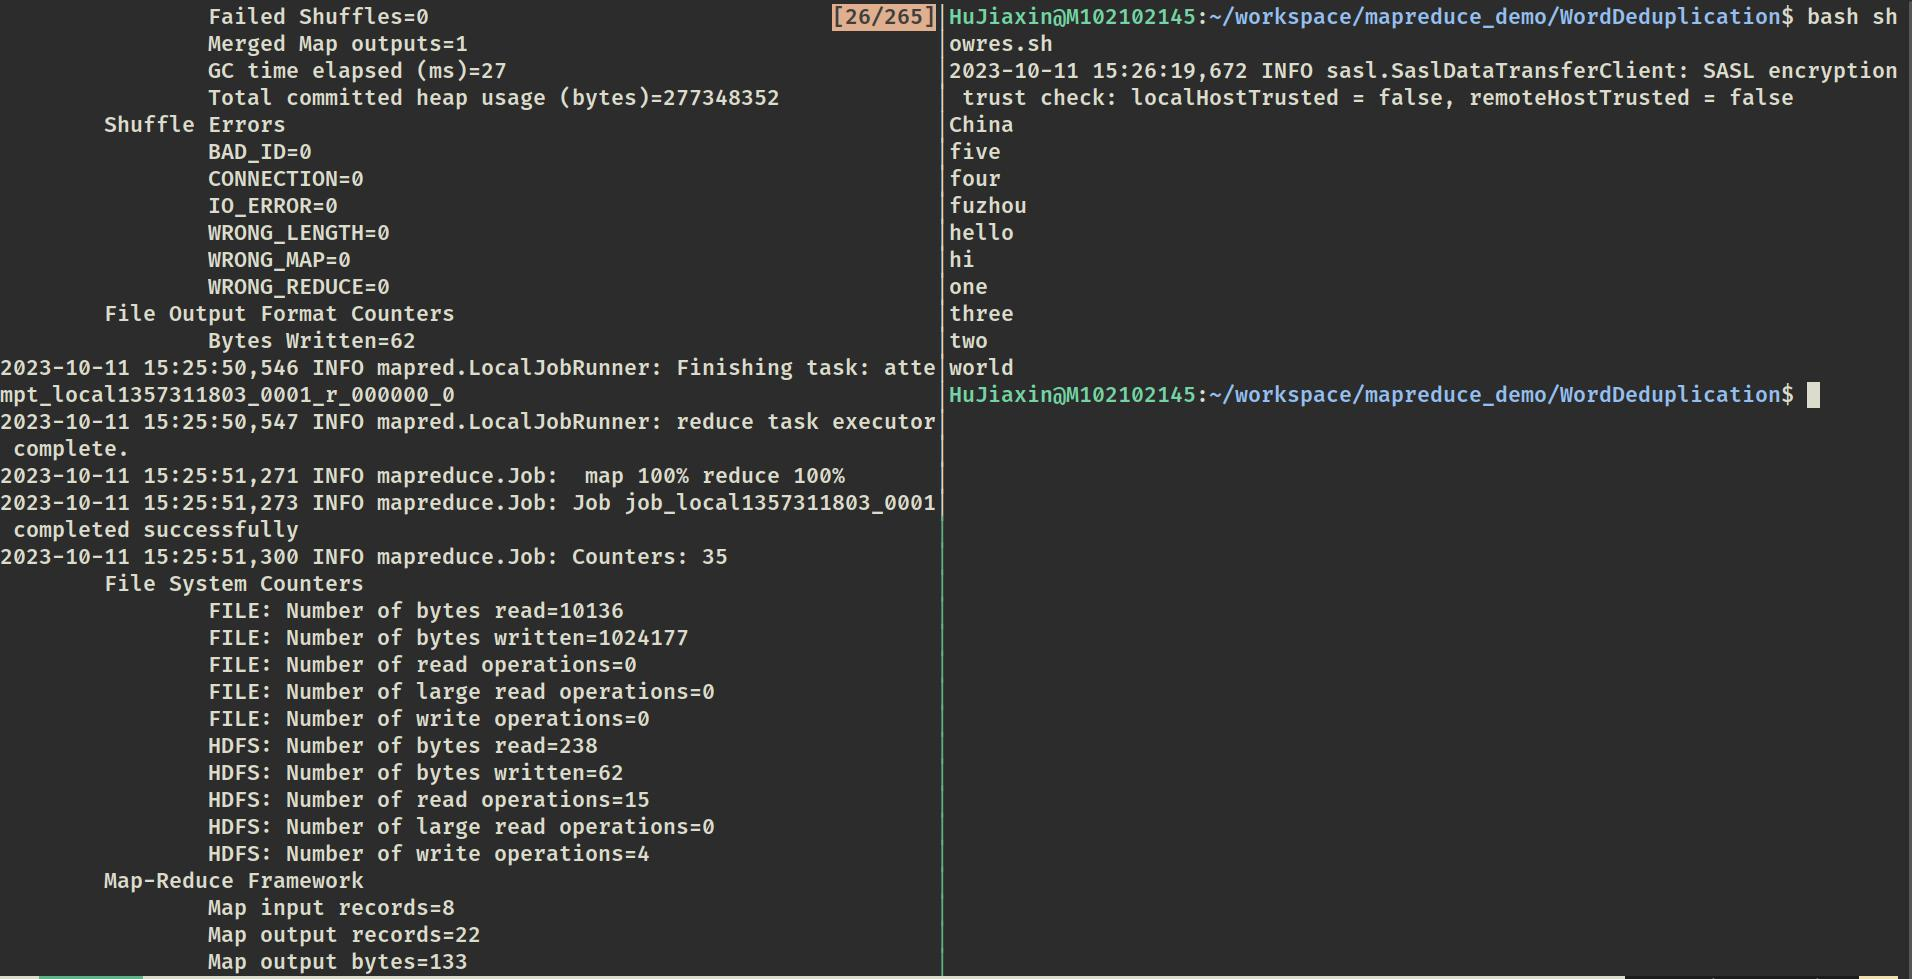
\includegraphics[width=0.95\textwidth]{./figures/1.jpg}
      \end{center}
      \caption{单词去重运行过程及其结果}
    \end{figure}


    \subsection{计算股票的资本损益}

    \subsubsection{Problem Description}

    描述: 统计买卖的每个股票收益.
    (将每个股票的名称作为 key 值, 当操作为 Buy 时, value 记为负的价格,
    当操作为 Sell 时, value 记为正的价格,
    以这个 key 和 value 作为 map 阶段输出, reduce 阶段的输入)

    \noindent Procedure:
    \begin{enumerate}
      \item 编写 MapReduce 代码;
      \item 编译并打包项目;
      \item 使用 hadoop jar 命令运行程序;
      \item 到控制台查看输出文件结果.
    \end{enumerate}

    \noindent Input:

    \noindent Leetcode Buy 1000 \\
    Corona Buy 10 \\
    Leetcode Sell 9000 \\
    Handbags Buy 30000 \\
    Corona Sell 1010 \\
    Corona Buy 1000 \\
    Corona Sell 500 \\
    Corona Buy 1000 \\
    Handbags Sell 7000 \\
    Corona Sell 10000

    \noindent Expected output:

    \noindent Corona Masks 9500 \\
    Handbags -23000 \\
    Leetcode 8000

    \subsubsection{Code}

    \begin{center}
\begin{minted}[xleftmargin=5mm]{java}
package net.homework;

import java.io.IOException;

import org.apache.hadoop.conf.Configuration;
import org.apache.hadoop.fs.Path;

import org.apache.hadoop.io.LongWritable;
import org.apache.hadoop.io.IntWritable;
import org.apache.hadoop.io.Text;

import org.apache.hadoop.mapreduce.Job;
import org.apache.hadoop.mapreduce.lib.input.FileInputFormat;
import org.apache.hadoop.mapreduce.lib.output.FileOutputFormat;

import org.apache.hadoop.mapreduce.Mapper;
import org.apache.hadoop.mapreduce.Reducer;

class AppMapper extends Mapper<LongWritable, Text, Text, IntWritable> {
  Text k = new Text(); // out-key
  IntWritable v = new IntWritable(); // out-val

  @Override
  protected void map(LongWritable key, Text value, Context context)
  throws IOException, InterruptedException {
    String line = value.toString();
    String[] arr = line.split(" ");
    String stockName = arr[0],
           status = arr[1],
           numStr = arr[2];

    int num = Integer.parseInt(numStr);
    if (status.equals("Buy")) {
      num = -num;
    }
    k.set(stockName);
    v.set(num);
    context.write(k, v);
  }
}

class AppReducer extends Reducer<Text, IntWritable, Text, IntWritable> {
  @Override
  protected void reduce(Text key, Iterable<IntWritable> values, Context context)
  throws IOException, InterruptedException {
    int sum = 0;

    for (IntWritable item : values) {
      sum += item.get();
    }

    context.write(key, new IntWritable(sum));
  }
}

public class StockCalculation {
  public static void main(String[] args)
  throws IOException, ClassNotFoundException, InterruptedException {
    Configuration conf = new Configuration();
    Job job = Job.getInstance(conf);

    job.setJarByClass(StockCalculation.class);

    job.setMapperClass(AppMapper.class);
    job.setReducerClass(AppReducer.class);

    job.setMapOutputKeyClass(Text.class);
    job.setMapOutputValueClass(IntWritable.class);

    job.setOutputKeyClass(Text.class);
    job.setOutputValueClass(IntWritable.class);

    FileInputFormat.setInputPaths(job, new Path(args[0]));
    FileOutputFormat.setOutputPath(job, new Path(args[1]));

    boolean result = job.waitForCompletion(true);
    System.exit(result ? 0 : 1);
  }
}
\end{minted}
    \end{center}

    \subsubsection{Result}

    \begin{figure}[H]
      \begin{center}
        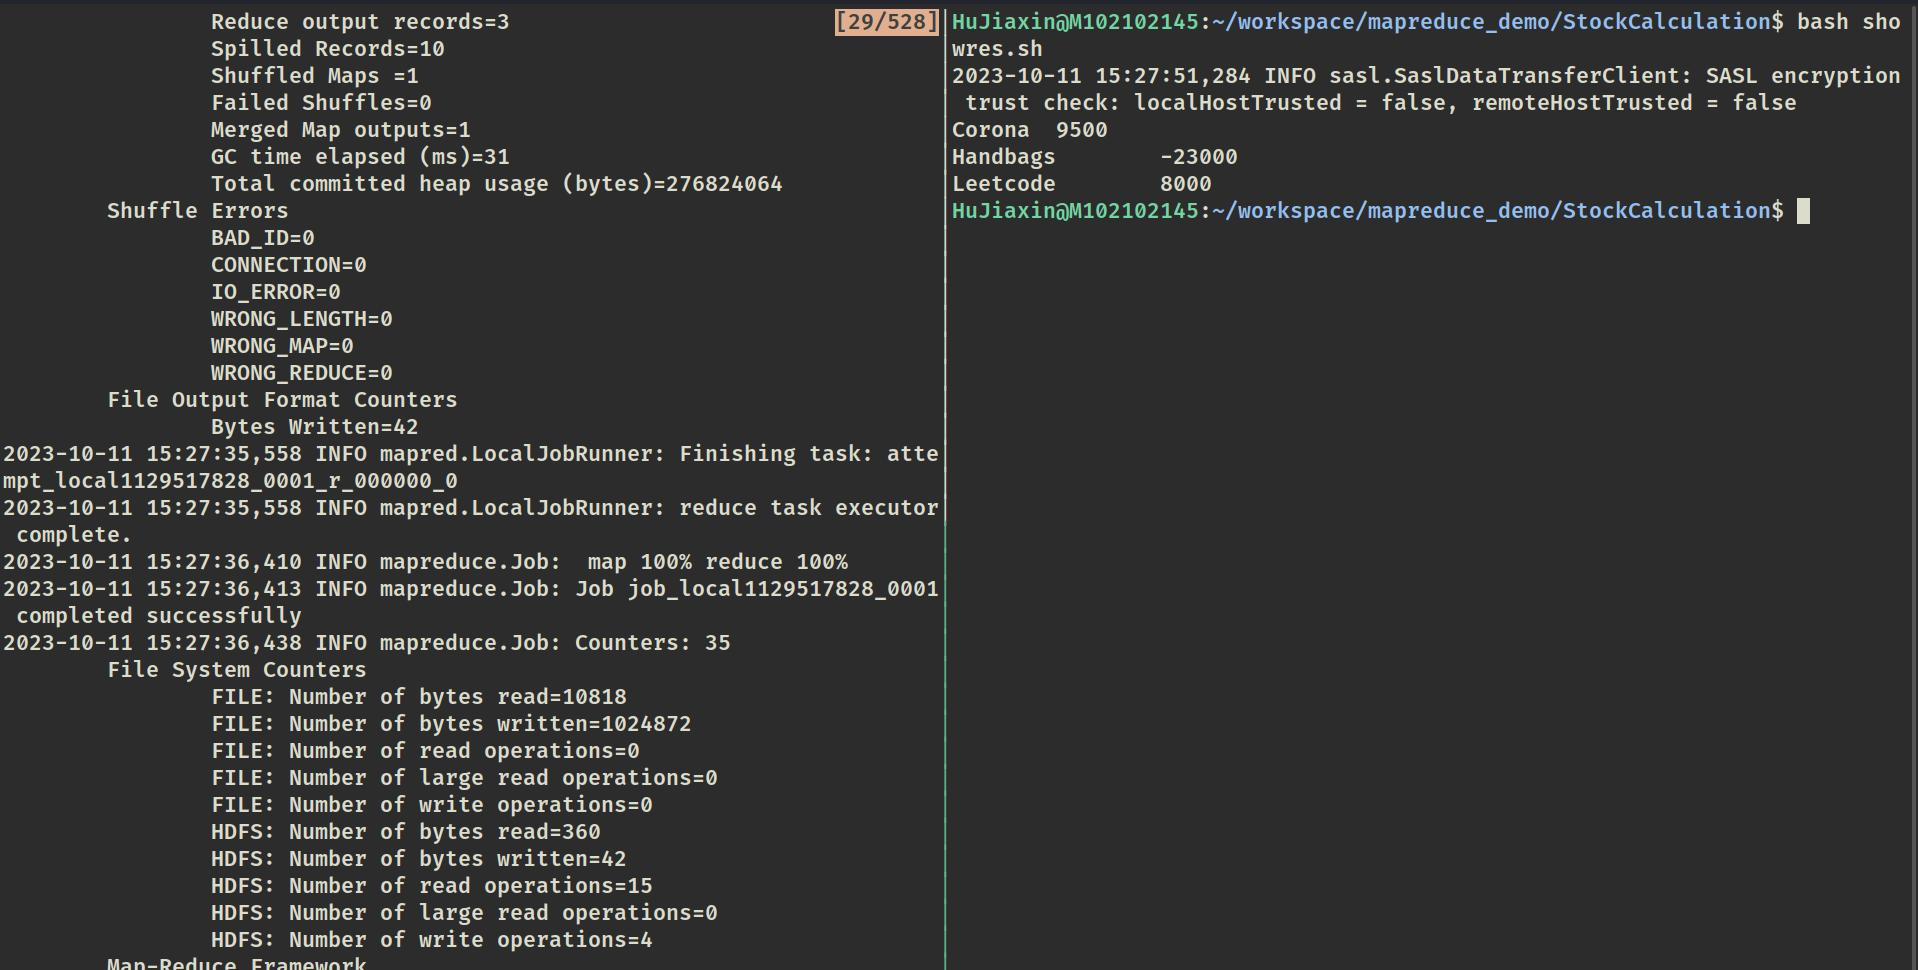
\includegraphics[width=0.95\textwidth]{./figures/2.jpg}
      \end{center}
      \caption{计算股票损益运行过程及其结果}
    \end{figure}

    \subsection{求互相关注的用户}

    \subsubsection{Problem Description}

    \noindent Procedure:
    \begin{enumerate}
      \item 编写 MapReduce 代码;
      \item 编译并打包项目;
      \item 使用 hadoop jar 命令运行程序;
      \item 到控制台查看输出文件结果.
    \end{enumerate}

    \noindent Input:

    \noindent A<B,C,D,F,E,O \\
    B<A,C,E,K \\
    C<F,A,D,I \\
    D<A,E,F,L \\
    E<B,C,D,M,L \\
    F<A,B,C,D,E,O,M \\
    G<A,C,D,E,F \\
    H<A,C,D,E,O \\
    I<A,O \\
    J<B,O \\
    K<A,C,D \\
    L<D,E,F \\
    M<E,F,G \\
    O<A,H,I,J,K

  如第一行表示用户 B,C,D,F,E,O 关注了 A, 现要求找出互相关注的所有用户
  对, 输出不能重复(输出了 A<->B 就不能输出 B<->A).

    \noindent Expected output:

    \noindent A<->B \\
    A<->C \\
    A<->D \\
    A<->F \\
    A<->O \\
    B<->E \\
    C<->F \\
    D<->E \\
    D<->F \\
    D<->L \\
    E<->L \\
    E<->M \\
    F<->M \\
    H<->O \\
    I<->O \\
    J<->O

    \subsubsection{Code}

    \begin{center}
\begin{minted}[xleftmargin=5mm]{java}
package net.homework;

import java.io.IOException;
import java.util.HashSet;
import java.util.ArrayList;
import java.util.Collections;

import org.apache.hadoop.conf.Configuration;
import org.apache.hadoop.fs.Path;

import org.apache.hadoop.io.LongWritable;
import org.apache.hadoop.io.Text;

import org.apache.hadoop.mapreduce.Job;
import org.apache.hadoop.mapreduce.lib.input.FileInputFormat;
import org.apache.hadoop.mapreduce.lib.output.FileOutputFormat;

import org.apache.hadoop.mapreduce.Mapper;
import org.apache.hadoop.mapreduce.Reducer;

class AppMapper extends Mapper<LongWritable, Text, Text, Text> {
  Text k = new Text(); // out-key

  @Override
  protected void map(LongWritable key, Text value, Context context)
  throws IOException, InterruptedException {
    String line = value.toString();
    String[] arr = line.split("<");
    String user = arr[0],
           fans = arr[1];
    String[] fansArr = fans.split(",");

    k.set(user);

    for (int i = 0; i < fansArr.length; i++) {
      if (user.compareTo(fansArr[i]) <= 0) {
        context.write(k, new Text(fansArr[i]));
      } else {
        context.write(new Text(fansArr[i]), k);
      }
    }
  }
}

class AppReducer extends Reducer<Text, Text, Text, Text> {
  @Override
  protected void reduce(Text key, Iterable<Text> values, Context context)
  throws IOException, InterruptedException {
    HashSet<String> set = new HashSet<String>();
    ArrayList<String> fansList = new ArrayList<String>();
    for (Text item : values) {
      String fan = item.toString();
      if (set.contains(fan)) {
        fansList.add(fan);
      } else {
        set.add(fan);
      }
    }
    Collections.sort(fansList);
    for (String item : fansList) {
        context.write(key, new Text(item));
    }
  }
}

public class FriendsFinder {
  public static void main(String[] args)
  throws IOException, ClassNotFoundException, InterruptedException {
    Configuration conf = new Configuration();

    conf.set("mapred.textoutputformat.ignoreseparator", "true");
    conf.set("mapred.textoutputformat.separator", "<->");

    Job job = Job.getInstance(conf);

    job.setJarByClass(FriendsFinder.class);

    job.setMapperClass(AppMapper.class);
    job.setReducerClass(AppReducer.class);

    job.setMapOutputKeyClass(Text.class);
    job.setMapOutputValueClass(Text.class);

    job.setOutputKeyClass(Text.class);
    job.setOutputValueClass(Text.class);

    FileInputFormat.setInputPaths(job, new Path(args[0]));
    FileOutputFormat.setOutputPath(job, new Path(args[1]));

    boolean result = job.waitForCompletion(true);
    System.exit(result ? 0 : 1);
  }
}
\end{minted}
    \end{center}

    \subsubsection{Result}

    \begin{figure}[H]
      \begin{center}
        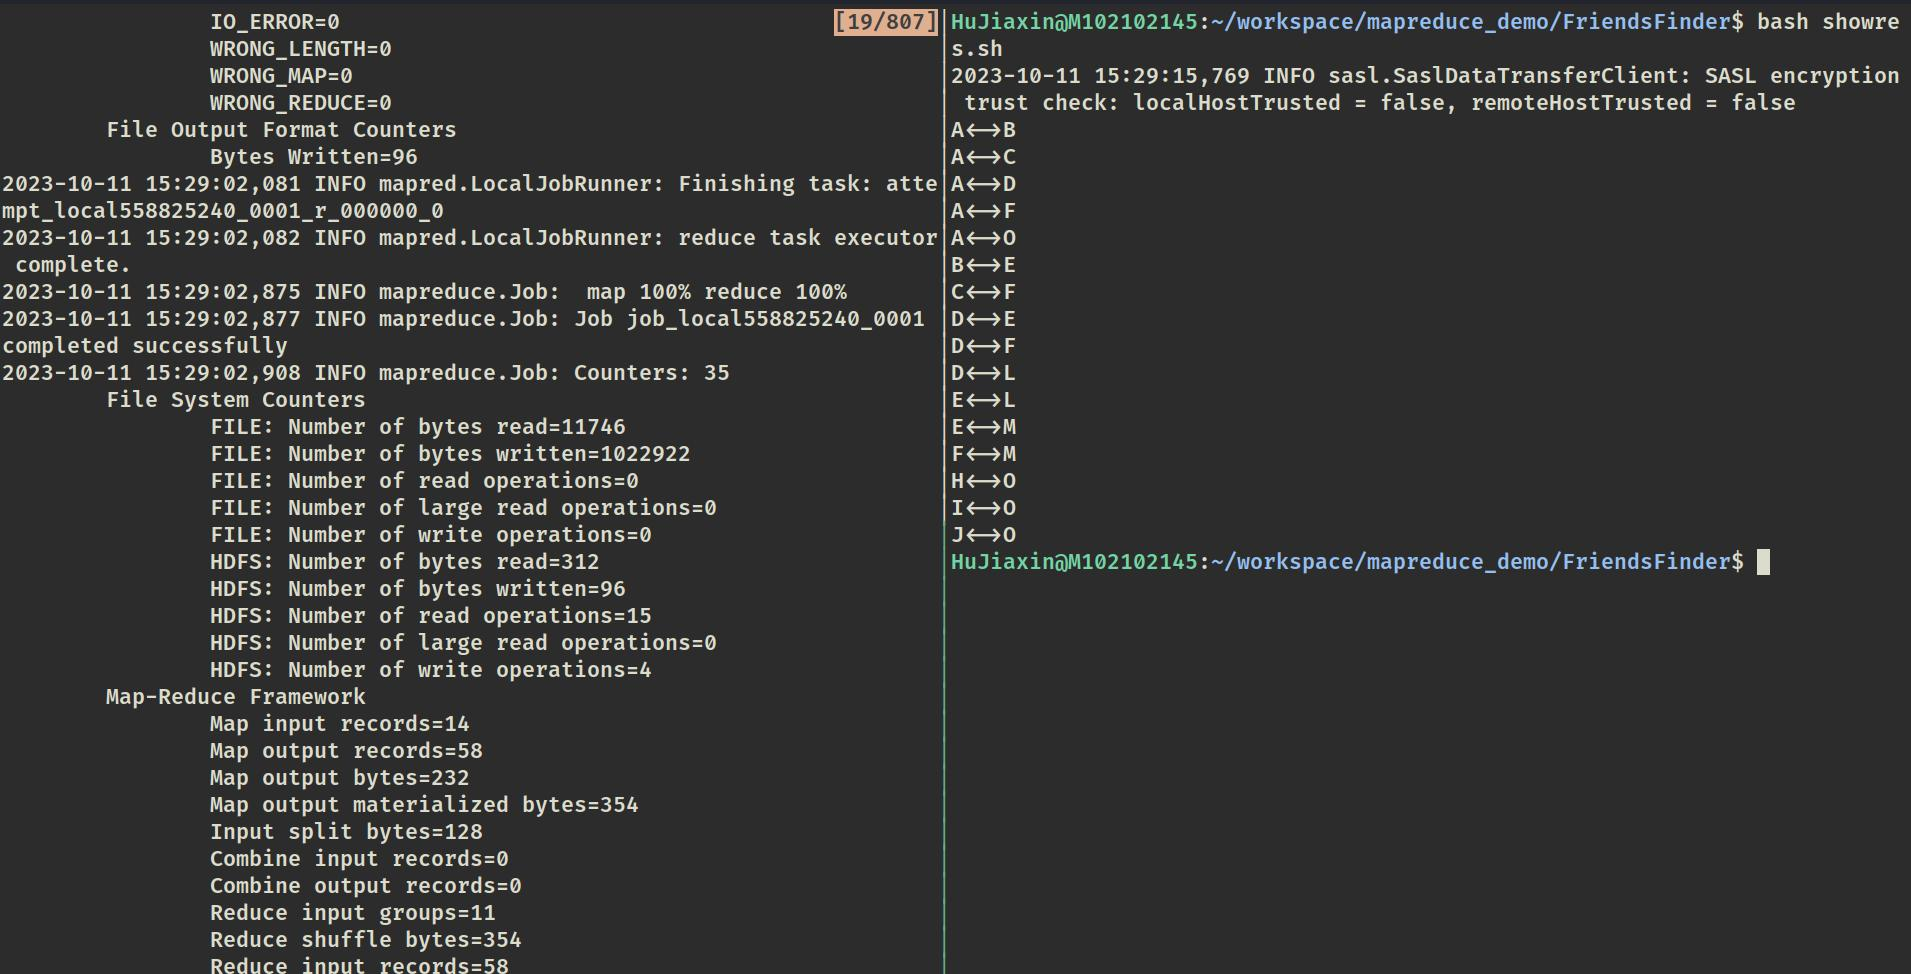
\includegraphics[width=0.95\textwidth]{./figures/3.jpg}
      \end{center}
      \caption{求相互关注的用户运行过程及其结果}
    \end{figure}

    \section{出现的问题及其解决方案}
    没有问题.
\end{document}
